
\documentclass[12pt,a4paper,english]{article}
\usepackage{graphicx, babel, csquotes, multicol, amssymb, fullpage}
\MakeOuterQuote{"}
\begin{document}

\title{Analysis of knowledge requirements for text alignment problem}
\author{Bartosz Kalińczuk}
\date{\today}
\maketitle

\newpage
\begin{abstract}
The purpose of this final master degree project was to experiment with various algorithms for speech and text alignment either with granularity of sentences, single words or even single phonemes. The output of this study was expected to find out how little data is necessary to compute a proper alignment. This project focuses mainly on Polish language, however it can be quite easily generalized for different languages. It also focuses solely on a audio with quite low level of noise, since  it introduces a lot of problems, and is out of the scope of this project.
\end{abstract}


\newpage
\setcounter{tocdepth}{2}
\tableofcontents

\newpage
\section{Introduction}

\newpage
\begin{center}
    \section{Speech signal}
\end {center}
\subsection{Human factor}

Speech is a most efficient way the human communicate. For generations this process was refined by evolution, so we can easily exchange messages even in hard situations. For this purpose our vocal mechanisms must well cooperate with our hearing ability. There is a certain set of sounds we can produce and our ears evolved to hear them as well as possible.\newline 

What is sound? According to dictionary: "Vibrations transmitted through an elastic solid or liquid or gas, with frequencies in the approximate range of 20 to 20000 hertz, capable of being detected by human organs of hearing". [1]\newline

How do we hear? Human ear consist about 30000 hair-cells, which can convert mechanical wave of the sound into electromagnetic wave inside auditory nerves [2]. 
Each of these cell is excited by different frequency of mechanical wave of internal ear fluids, so it is no surprise, that people can hear only a certain range of frequencies, as stated in definition. These we expect to be finely tuned to the range of the sounds we can produce. Although it seems, that we can hear a bit more, but as we don't need that, it happens, that as we grow older, our hearing range is getting smaller, because our hear cells fail sometimes, but mostly those responsible for high frequencies, which we don't use too often.\newline

Humans can hear frequencies, that begins as low as 12Hz (under laboratory conditions) to 20kHz (for adults usually much lower). However speech range is a little bit smaller than that [3]: \newline

\begin{center}
    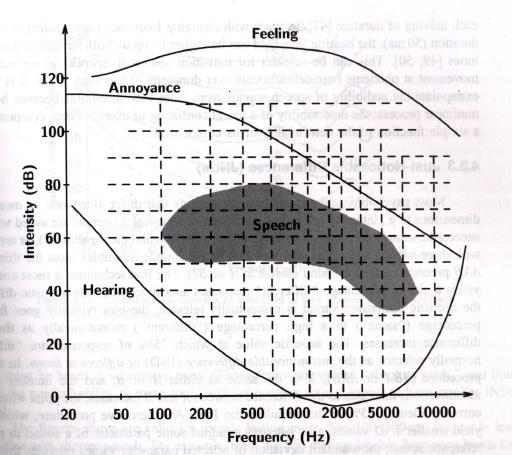
\includegraphics[scale=0.5]{speech_range.jpg}
\end {center}


\newpage
\subsection{Mel scale}

How we perceive sound, that is completely different matter and topic for long philosophical discussion. However we can help ourselves with some subjective experiments. For example Stevens, Volkman and Newman conducted an experiment on a number of listeners to measure, what do we perceive as equally distanced pitches. In this experiment, the participants of the experiment were asked to judge if given pitches were in equal distances. The output was, that humans don't experience sound linearly respectively to the frequency scale, but a perceptual scale was closer to logarithmic one. [5] \newline

Certain formulas were conceived to translate frequency scale to one, that is closer to how human actually perceive sound. \newline

One popular is mel scale, where mel comes from melody: [6] \newline
\begin{equation}
    m = 2595log_{10}(1 + \frac{f}{700})
\end{equation}
	
What looks like that:
\begin{center}
    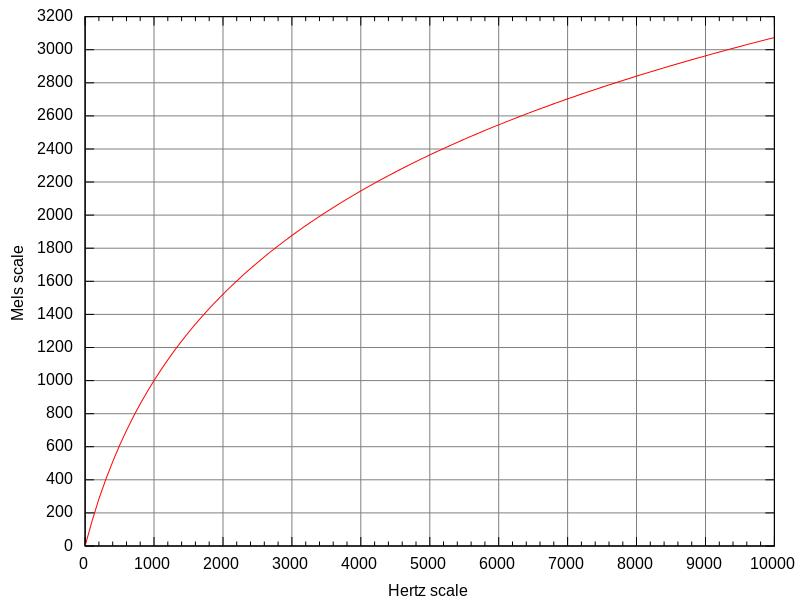
\includegraphics[scale=0.3]{mel_scale.jpg}
\end {center}

Another popular formula of so called bark scale, which is based on perception of loudness of the sound and proposed by Eberhard Zwicker in 1961. [7] \newline
\begin{equation}
    Bark = 13 atan(\frac{0.76f}{1000}) + 3.5 atan(\frac{f^2}{7500^2})
\end{equation}
In this project we use mel scale implemented in sphinx library, although bark scale is becoming more popular recently.

\newpage
\subsection{Frequency spectrum}

The conclusion from the anatomy of human ear is, that frequencies of the sound are important.
How can we obtain frequency spectrum from a digitized sound, so we can proceed further? \newline
The obvious tool for conversion of discrete function to frequencies is Discrete Fourier Transform, named after Jean Baptiste Joseph Fourier it is one of the most often used techniques of modern times. \newline

It all started from the postulate, that a heat equation can be satisfied by function of form: [11] \newline
\begin{equation}
    f(x)=\sum_{n=0}^N(A_n cos(nx) + B_n sin(nx))
\end{equation}
or in complex form:
\begin{equation}
    f(\theta)=\sum_{n=-\infty}^{\infty} C_n e^{i n \theta}
\end{equation}

Basically we convert our function's domain to frequency domain or to domain of sinusoidal functions. $C_n$ coefficients are complex values that encode both amplitude and phase of the converted signal/function at each frequency. \newline

The coefficients for any integrable functions over an interval $[\frac{-T}{2}, \frac{T}{2}]$ can be obtain using formula: [11] \newline
\begin{equation}
    C_n=\int_{\frac{-T}{2}}^{\frac{T}{2}} f(x) e^{-2 \pi i \frac{n}{T} x} dx
\end{equation}

or for the discrete case:
\begin{equation}
    C_k=\sum_{n=0}^{N-1} x_n e^{\frac{-2 \pi i k n}{N}} dx
\end{equation}
	

So far we haven't found any use in the speech recognition for phase part of the coefficients, however amplitude determines how powerful is signal at given frequency. The power value is given by:
\begin{equation}
    |X_k|/N = \sqrt{\Re(X_k)^2 + \Im(X_k)^2} / N
\end{equation}

\newpage
A sample conversion:
\begin{center}
    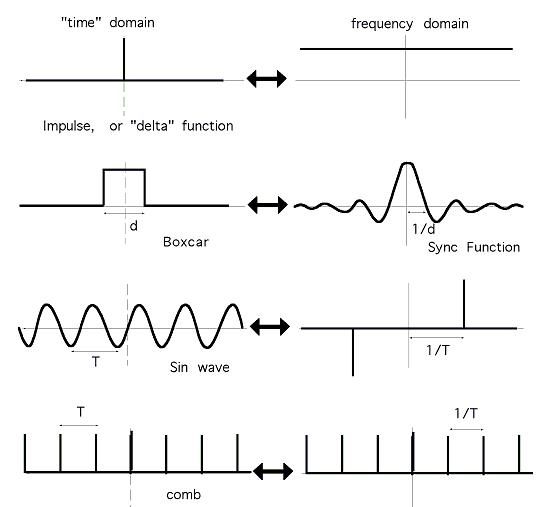
\includegraphics[scale=0.3]{sample_dft_conversion.jpg}
\end {center}

What size of the window should we use? First we have to notice, that in order to capture certain frequency, the window needs to be large enough. We would like to examine signals of frequency ranged from 100Hz (see speech frequencies ranges in chapter 2.1), which is a period of 100th of the second, so a 10millisecond window would be our bottom limit. \newline

Also windows with abrupt signal discontinuities may cause result with spectral artefacts, so a windowing function is usually applied. Popular choice is a Hamming window function: [8]
\begin{equation}
   w_j = 0.54 - 0.46 cos(\frac{2 \pi j}{W - 1}) 
\end{equation}
Which's plot is:
\begin{center}
    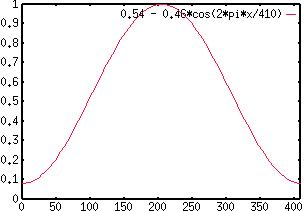
\includegraphics[scale=0.3]{hamming_window.jpg}
\end {center}

Note that it emphasises values in the middle of the window, so our actual windows should overlap to cover whole time domain. For example by shifting a window by a percentage of it actual width:
\begin{center}
    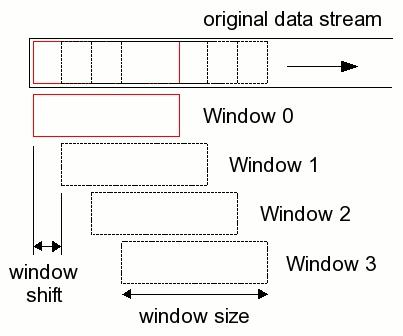
\includegraphics[scale=0.3]{window_shifting.jpg}
\end {center}

\newpage
A human speech signal in frequency and time domain: [3]
\begin{center}
    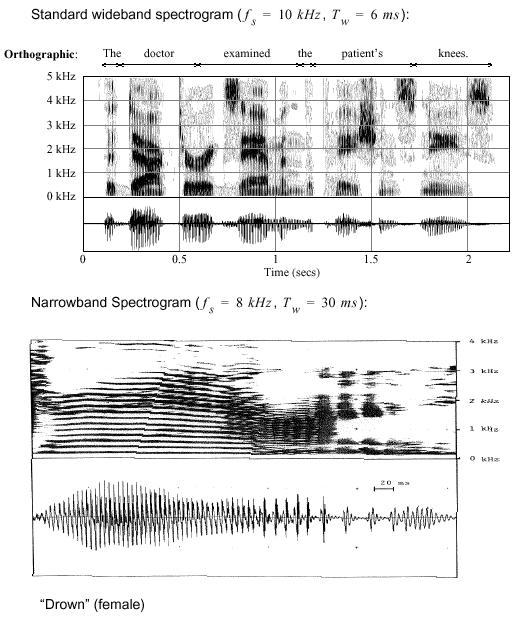
\includegraphics[scale=0.8]{speech_spectrogram.jpg}
\end {center}

\newpage
\subsection{Cepstrum}

Looking at the frequency spectrum of human speech we see, that  the signal in the frequency domain contain features that are quite periodic. As it is with converting initial signal with DFT, we would like to extract the information of periodicity in the spectrum. 
A cepstrum of the signal gives us this additional information. \newline

The word is derived by reordering characters in the word spectrum to indicate switch of domains, similarly as word 'quefrency'. The cepstrum operates in the domain of time and the basic intuition is, that it reveals a rate of change in the different spectrum bands. 
For example a cepstrum of an echoed signal in the picture below shows clearly a three 'quefrencies' of the echo of the signal. [12]
\begin{center}
    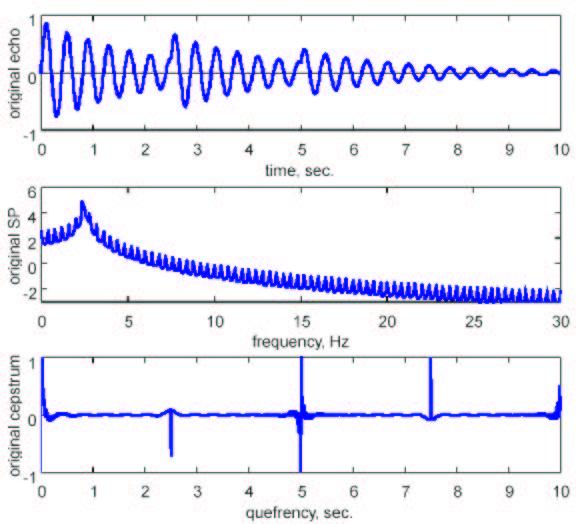
\includegraphics[scale=0.4]{echo_cepstrum.jpg}
\end {center}


Cepstrum definition is: "Inverse Fourier transform of the logarithm of the magnitude of the Fourier transform" or:
\begin{equation}
    C=|F^{-1}{log(|F{f(t)}|^2)}|^2
\end{equation}

,or:
\begin{equation}
    c_x[n] = \frac{1}{2\pi} \int_{-\pi}^{\pi}log |X(e^{j \omega})| e^{j \omega n} d\omega
\end{equation}

This is the definition of the power cepstrum, since it is calculated from the magnitude of each frequency band. However there also exists a complex, real and phase cepstrum depending on what part of initial Fourier transform it uses.
In speech related problems a power cepstrum is usually used and I haven't see any reason to not focus only on this.


\newpage
\addtolength{\textwidth}{4cm}
This is a typical cepstrum sequence of the vowel [3] computed every 10ms. \newline

\begin{minipage}[-100,0]{5cm}
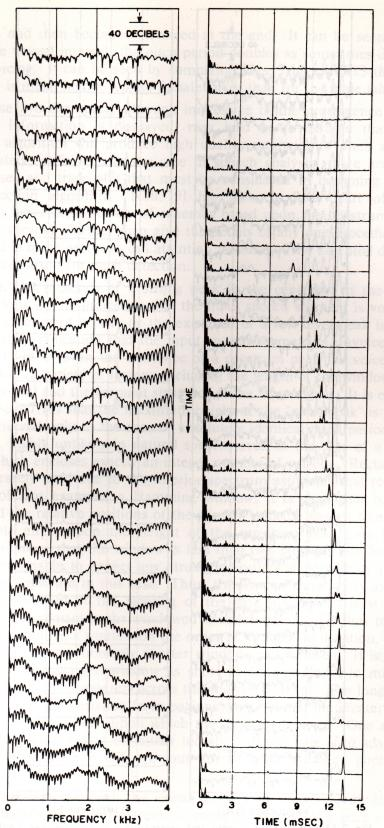
\includegraphics[width=5cm,height=21cm]{vowel_cepstrum.jpg}
\end{minipage}
\begin{minipage}[5cm,0]{9cm}

If the sound becomes periodic in the frequency domain it's quefrency domain contains a peak which is related to the periodicity of the sound. \newline

Note that similar results can be obtained by taking just additional DFT of the signal. Inverse Fourier Transform is closely related to Fourier Transform and also performs a split of the function into periodic components. \newline
\newline
After all IFT is defined:
\begin{equation}
     f(x) = \int_{\mathbb{R} ^ n} e^{2 i \pi x \zeta} \hat{f}(\zeta) d\zeta
\end{equation}
while FT is defined: 
\begin{equation}
    \hat{f}(\zeta) = \int_{\mathbb{R} ^ n} f(x) e^{-2 i \pi \zeta x} dx
\end{equation}

Why taking logarithm of the magnitude? It serves as a normalization of power spectrum. In speech for example it happens, that low frequency components are usually more powerful than high frequncy components and by normalizing the signal, the periodicity becomes more apparent. \newline


A bit different way of looking at the signal cepstrum is as a homomorphic transformation which changes convolution into sum. [3]
\begin{equation}
x(n) = e(n) * h(n)
\end{equation}
\begin{equation}
\hat x(n) = \hat e(n) + \hat h(n)
\end{equation}


Which on it's own can be seen as way of separating signals, since it is more easy to extract elements from a sum, than from a convolution.
\newline
\newline
In the example with echo, we could have used the cepstrum to separate echoed signal from initial signal, and it might be used to filter out an audio feedback.

\end{minipage}

\newpage
\subsection{Sphinx frontend}


Sphinx is a speech recognition toolkit with a lot of useful functionalities for any speech related problem.  \newline
There is a certain common way to prepare a speech signal for the further processing. With slight variations in each step, the useful informations about speech are drawn from a cepstrum of the reduced signal (in the number of data dimensions), as presented in this chapter. \newline

In order to skip the reinvention of the wheel, I used the fronted part of the sphinx library in any experiment in this project.
The sphinx fronted performs signal transformation and produces data composed of only 39 voice features,
while actually only 13 are base ones and the rest is a derivation of these. \newline

Sphinx frontend is a list of transformations executed on the result of the transformation placed higher in the list.
In another words it is a transformation composition. \newline
\newline
This Sphinx frontend pipeline includes: \newline
\begin{itemize}
	\item Data Blocker,
	\item Preemphasizer,
	\item Windower,
	\item Discrete Fourier Transform,
	\item Mel Frequency Filter Bank,
	\item Discrete Cosine Transform,
	\item Cepstral Mean Normalization,
	\item Deltas Feature Extractor.
\end{itemize}

\subsubsection{Data Blocker}

This initial transformation reads incoming double data read from audio source (file or microphone) and
prepares blocks of the data to be used in later phases. In our case blocks contain 10ms of audio data.

\subsubsection{Preemphasizer}

The Preemphasizer applies a formula: $Y[i]=x[i]-(X[i-1] * preemphasizerFactor)$.
The purpose of this transformation is to emphasize the high frequency components. It is kind of filter,
which allows high frequency components to pass through, but weakens the low frequency ones.


\newpage
\subsubsection{Raised cosine windower}

Creates windows from the incoming data. A windowing function
\begin{equation}
    W(n)=(1-\alpha) - \alpha cos(\frac{2 \pi n}{N - 1})
\end{equation}
 is applied afterwards. Alpha coefficient set to 0.46 results with a mentioned before Hamming windowing
 function, which is a default setting and the one used by me.

\subsubsection{Discrete Fourier Transform}

Implementation of fast Fourier transform .The FFT can perform transformation with complexity $\Omega(Nlog(N))$,
where N is the size of the input data.
It can be perform on whole data, however in speech we would like to get an information of the frequencies 
of a small frame, that contains consistent speech signal, in particular a single phoneme.
The output data is the power spectrum of input data window and the complex/phase information is lost.
The number of FFT points is the closest power of 2 equal or larger to the number of samples in the incoming window of data. However the input signal is real, so resulting FFT is symmetric, so only half of the data is returned and the output size is $\frac{FFT points}{2} + 1$.

\subsubsection{Mel frequency filter bank}

This step is a part of calculating a Mel Frequency Cepstrum. \newline

Conversion of frequency spectrum into a mel-spectrum using triangular overlapping windows defined as:
\begin{equation}
    w(n) = 1 - |\frac{n - (N - 1)/2}{(N + 1)/2}|
\end{equation}


The number of triangles/filters defined the size of mel-spectrum and the sphinx's default is 40. \newline
The filters are chosen, so the result would simulate a mel-scale given by the formula:
\begin{equation}
    melFreq = 2595 log(1 + linearFrequency / 700)
\end{equation}

The given filters should look like in the picture:
\begin{center}
    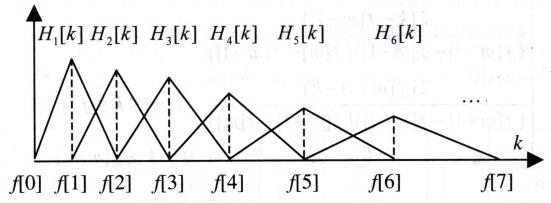
\includegraphics[scale=0.4]{mel_filters.jpg}
\end {center}

Not all frequencies are covered by the filters.
The chosen range of frequencies may differ for various audio encodings,
but generally should cover only the speech ranges.
The default values for 16kHz sample rate streams are 130Hz-6800Hz and are not changed in this project.

\newpage
\subsubsection{Discrete Cosine Transform}

Another part of calculating Mel Frequency Cepstral Coefficient vector.  \newline

It applies a logarithm and the DCT type II to the input data.  \newline

A DCT type II (most common) coefficients are defined as: 
\begin{equation}
    C(u) = \alpha(u)\sum_{x=0}^{N-1} f(x)cos[\frac{\pi(2x+1)u}{2N}] 
\end{equation}
and it is quite tightly related to real part of the Fourier Transform. [18]
The transform represents a function as a sum of cosine functions and it is equivalent to the DFT operating
real data with even symmetry. \newline
The number of dimensions returned is set by default to 13.

\subsubsection{Cepstral Mean Normalization}

Performs a normalization of MFCC vector by subtracting a mean of all the input. There are two versions
of this step. One that calculates mean online and the other that reads all data before performing
subtraction.

\subsubsection{Deltas feature extractor}

The final transformation in the sphinx frontend chain. It calculates first and second order derivative of the
cepstrum as additional features of the speech signal. It improves noticeable speech processing algorithms
by adding additional information about changes in the cepstrum data. \newline

For the initial cepstrum data it adds additionally twice the size vector with first and second order
differences, calculated as shown in the picture:
\begin{center}
    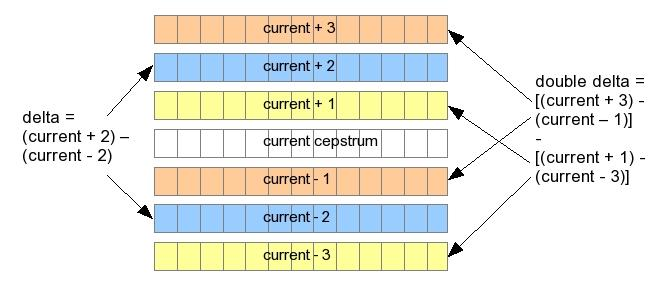
\includegraphics[scale=0.6]{deltas_calc.jpg}
\end {center}


\end{document}
